\maketitle

This problem set is due on Wednesday, April 26 at 11:59 pm. Each problem part is worth 3 points. Collaboration is encouraged. In all cases, you must write your own solutions, and and you must cite collaborators and resources used.

\begin{problem}
The Wolfram Mathematica reference page on the \texttt{ComplexPlot} Mathematica function includes this helpful interpretation guide:
\begin{center}
  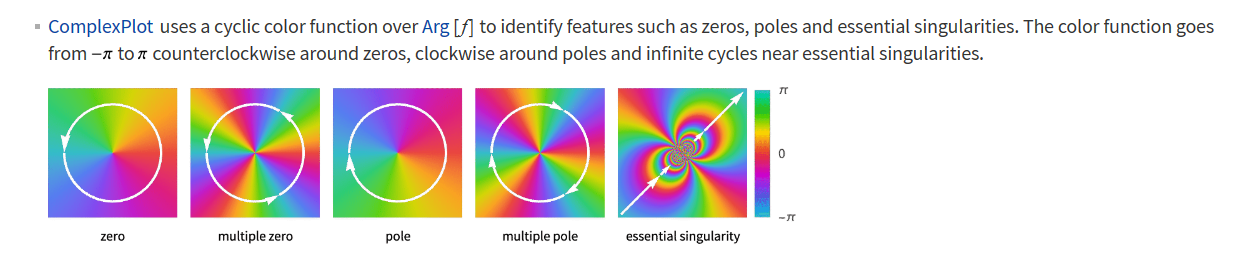
\includegraphics[width=\textwidth]{screenshot.png}
\end{center}
\begin{enumerate}[(a)]
  \item First, you should prove that the guide is correct, at least for zeros and poles. Let $f$ be a holomorphic function and let $a$ be either an isolated zero or isolated pole of $f$. Let $\gamma$ be a counterclockwise loop around $a$ such that $a$ is the only zero or pole in or on $\gamma$. Prove that
  \[\int_\gamma d\arg(f(z))\footnote{Even though $\arg$ is multi-valued, integrating $d\arg(f(z))$ over a curve is well defined because the end point minus starting point of the image curve $\arg(f(\gamma))$ is unique. This goes for $d\log(f(z))$ as well.}\]
  equals $2\pi$ times $\ord_a f$.

  \emph{Hint:} Here are some steps:
  \begin{itemize}
    \item Write $f(z)$ as $|f(z)|e^{i\arg(f(z))}$, the polar form decomposition of the output of $f$, valid over $\gamma$ since $f(z)$ lies in $\bC-\{0\}$ for $z\in\gamma$.
    \item Deduce that $\arg(f(z))=\frac 1i(\log(f(z))-\log|f(z)|)$.
    \item Argue that $\int_\gamma d\log|f(z)|=0$ because $\log|f(z)|$ for $z\in\gamma$ describes a closed path on the real axis, so must return to its initial value.
    \item Finish with the argument principle.
  \end{itemize}

  \item Explain how part (a) proves the correctness of the guide in the image in the first four cases.
  
  \item Fire up a plot of $\zeta(z)$ on your favorite complex plotter on the internet. (Typing \texttt{zeta(z)} should work to input the function.) Find as many zeros or poles of this function as you can and classify them using the guide (along with their orders). For the zeros that aren't on the real axis, what do you notice about their real parts? Any conjecture?
\end{enumerate}
\end{problem}

\begin{problem}
  Let $f(s)=\zeta(s)\cdot\zeta(s)$, the product of the Riemann zeta function with itself. If we write
  \[f(s)=\sum_{n=1}^\infty\frac{a_n}{n^s}\]
  for some integers $a_n$, prove that $a_n=d(n)$, the number of divisors of $n$. Cool!
\end{problem}

\begin{problem}
  A very popular Numberphile meme is that
  \[1+2+3+\cdots=-\frac 1{12}.\]
  Finally you get to see where this comes from.
  \begin{enumerate}[(a)]
    \item Explain informally why $\zeta(-1)$ is a natural replacement for the divergent sum $1+2+3+\cdots$.
    \item Compute $\zeta(-1)$ using equation (59) on page 214 of Ahlfors, and show that it is equal to $-1/12$. You may find the argument in the proof on the beginning of page 215 helpful. Note well that the integral over the circular part of $C$ is \emph{not} zero in this case --- it is zero in the proof because, in the context of the theorem, we had $\Re s>1$.
    
    You may freely use the fact that the first few terms of the Laurent series of $1/(e^z-1)$ around $z=0$ is
    \[\frac 1z-\frac12+\frac z{12}-\frac{z^3}{720}+\cdots.\]
  \end{enumerate}
\end{problem}

\begin{problem}
  What is your favorite theorem or method from this class?
\end{problem}

\begin{problem}
This is a space to reflect on something about this problem set. You can mention if you found any problems particularly difficult, or particularly easy. You can also mention problems you liked, or problems that took a long time, etc. (Please write something here to get credit!)
\end{problem}
